\documentclass[11pt,a4paper]{ivoa}
\input tthdefs

\usepackage{xspace}
% Standard terms used throughout the document,
% defined as macro commands to maintain consistency
\newcommand{\xml} {XML\xspace}
\newcommand{\json} {JSON\xspace}
\newcommand{\yaml} {YAML\xspace}
\newcommand{\webservice} {webservice\xspace}

\newcommand{\uws} {UWS\xspace}
\newcommand{\uwsce} {UWS-CE\xspace}

\newcommand{\ivoa} {IVOA\xspace}
\newcommand{\execplan} {Execution Planner\xspace}
\newcommand{\ivoaexecplan} {IVOA Execution Planner\xspace}

\newcommand{\docker} {Docker\xspace}
\newcommand{\dockercompose} {Docker Compose\xspace}

\newcommand{\binderhub} {BinderHub\xspace}
\newcommand{\jupyter} {Jupyter\xspace}
\newcommand{\jupyterhub} {JupyterHub\xspace}
\newcommand{\jupyternote} {Jupyter notebook\xspace}

\newcommand{\esap} {ESAP\xspace}
\newcommand{\escape} {ESCAPE\xspace}
\newcommand{\datalake} {DataLake\xspace}
\newcommand{\rucio} {Rucio\xspace}

\newcommand{\python} {Python\xspace}
\newcommand{\pythonprog} {Python program\xspace}

\newcommand{\apache} {Apache\xspace}
\newcommand{\spark} {Spark\xspace}
\newcommand{\pyspark} {PySpark\xspace}
\newcommand{\zeppelin} {Zeppelin\xspace}
\newcommand{\zeppelinnote} {Zeppelin notebook\xspace}

\newcommand{\codeword}[1] {\texttt{#1}}
\newcommand{\footurl}[1] {\footnote{\url{#1}}}

\newcommand{\dataset} {dataset\xspace}
\newcommand{\scienceplatform} {Science Platform\xspace}

\title{IVOA Execution Planner}

% see ivoatexDoc for what group names to use here; use \ivoagroup[IG] for
% interest groups.
\ivoagroup{GWS}

\author[http://www.ivoa.net/twiki/bin/view/IVOA/DaveMorris]
       {Dave Morris}

\editor[http://www.ivoa.net/twiki/bin/view/IVOA/DaveMorris]
       {Dave Morris}

% \previousversion[????URL????]{????Concise Document Label????}
\previousversion{This is the first public release}


\begin{document}
\begin{abstract}

One of the long term goals of the IVOA has been to enable users to
\textit{`move the code to the data`}.
As the size and complexity of the \dataset{}s available in the VO increases
this is becoming more and more important.

The \ivoaexecplan provides a step towards making this possible.

The \ivoaexecplan is designed to address a specific question;
given an \textit{`executable thing`}, e.g. a \pythonprog or \jupyternote,
what facilities are available to run it?

To do this, the \ivoaexecplan specification defines two components;
a data model for describing an executable program
and the resources needed to execute it,
and a \webservice API for querying the VO to find services
that are able to execute it.

Together these components enable a user to ask a simple question
\textit{"Where (and when) can I execute my program?"}

This in turn enables \scienceplatform{}s to share code between different platforms.
Allowing a user to develop their code on one platform and then apply it to a different
\dataset by sending it to execute on another platform.

\end{abstract}

\section*{Acknowledgments}

The authors would like to thank all the participants in the IVOA and ESCAPE projects
who have contributed their ideas, critical reviews, and suggestions to this document.

\section*{Conformance-related definitions}

The words ``MUST'', ``SHALL'', ``SHOULD'', ``MAY'', ``RECOMMENDED'', and
``OPTIONAL'' (in upper or lower case) used in this document are to be
interpreted as described in IETF standard RFC2119 \citep{std:RFC2119}.

The \emph{Virtual Observatory (VO)} is a general term for a collection of
federated resources that can be used to conduct astronomical research,
education, and outreach.
The \href{https://www.ivoa.net}{International Virtual Observatory Alliance (IVOA)}
is a global collaboration of separately funded projects to develop standards and
infrastructure that enable VO applications.

\section{Introduction}

???? Write something ????

\subsection{Role within the VO Architecture}

\begin{figure}
\centering

% As of ivoatex 1.2, the architecture diagram is generated by ivoatex in
% SVG; copy ivoatex/archdiag-full.xml to role_diagram.xml and throw out
% all lines not relevant to your standard.
% Notes don't generally need this.  If you don't copy role_diagram.xml,
% you must remove role_diagram.pdf from SOURCES in the Makefile.

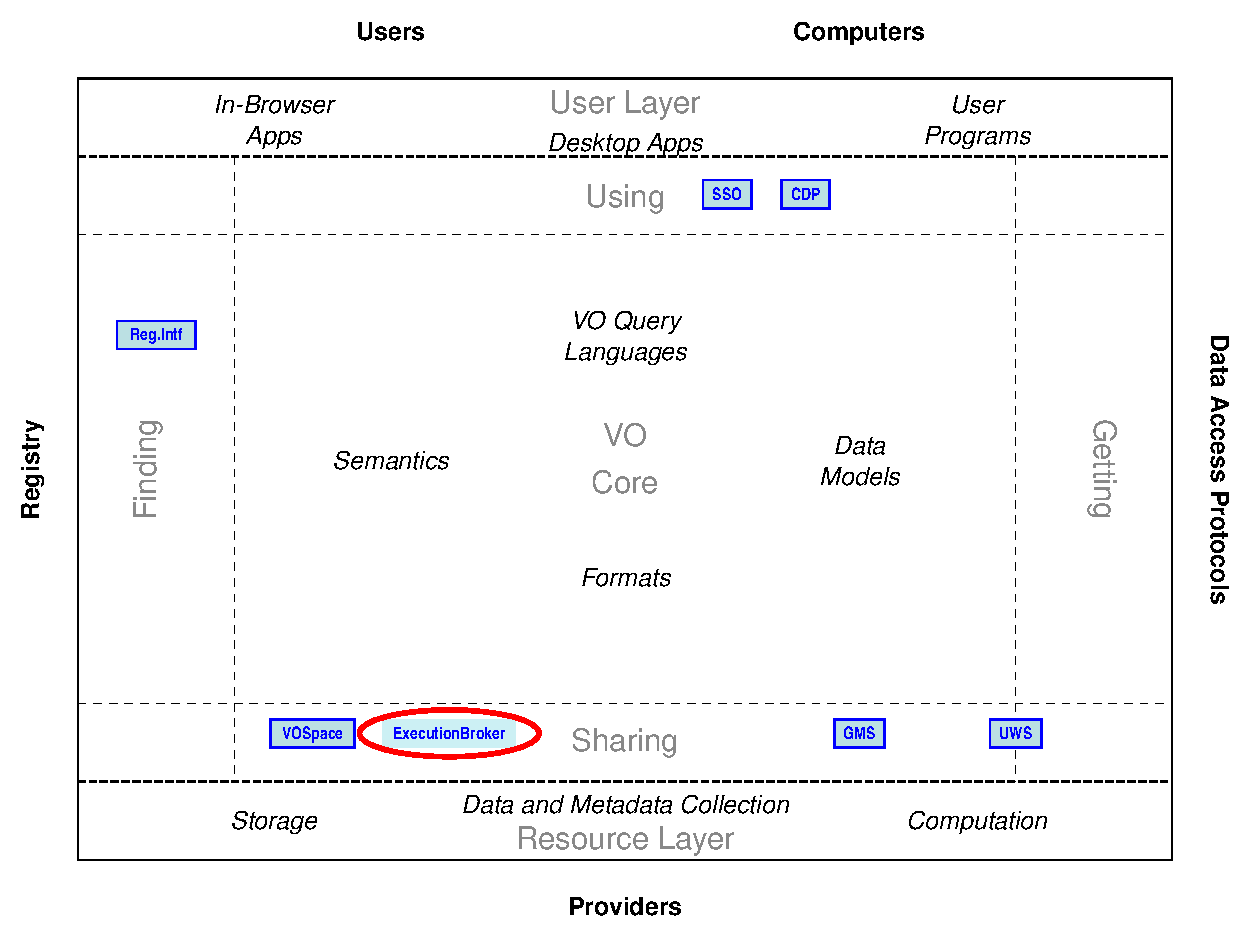
\includegraphics[width=0.9\textwidth]{role_diagram.pdf}
\caption{Architecture diagram for this document}
\label{fig:archdiag}
\end{figure}

Fig.~\ref{fig:archdiag} shows the role this document plays within the
IVOA architecture \citep{2021ivoa.spec.1101D}.

???? and so on, LaTeX as you know and love it. ????

\appendix
\section{Changes from Previous Versions}

No previous versions yet.
% these would be subsections "Changes from v. WD-..."
% Use itemize environments.


% NOTE: IVOA recommendations must be cited from docrepo rather than ivoabib
% (REC entries there are for legacy documents only)
\bibliography{ivoatex/ivoabib,ivoatex/docrepo}


\end{document}
